\chapter{Search by Face Similarity}
\label{ch:face_search}

In this chapter, we propose another approach to the CBIR task. In this approach, we search only over the part of the dataset, which contains people. We ask if it is possible to find the target image based on the face of the person and faces of other people in the dataset.

This question arises from practical reasons. Once we investigated the V3C1 dataset, we realized that many of the images display people. We can use the previously investigated approaches based on the location and visual similarity to find the target image. However, with the increasing number of images showing people, it becomes difficult to retrieve the correct target image. Also, finding a good representative faces with similar background becomes a challenging task.

The technique described in this chapter works only on the feature space of faces. We first extract the faces from the dataset, and then we obtain a representation for each one of them. Based on these representations, we organize the faces into a traversal structure supporting navigational commands.

The task of comparing the faces of the people and saying which look more similar has its roots in the human perception of the faces. Therefore, to evaluate the individual steps, we conduct experiments with real users.

Our experiments show that the feature space of the descriptors has limited power to order people based on the similarity in a way people do. Despite that, we implement the traversal structure, which can be used with any new representation of the faces that could be developed in the future. Our last evaluations show that the median of the time required to find the target scene was smaller for our traversal approach than the baseline -- linear search.

\section{Extraction of the faces}

Face Detection is a widely studied problem. One of the key advancements in the past in this are was an article by \ref{} the authors improved the human detection using Histogram of oriented gradients descriptor methods. The method is quick enough to perform even online. The disadvantage of the approach its lower performance on non-frontal views of the faces. Even today it is sometimes preferred due to its efficiency.

Another, recently common approach, is to use a CNN based approach for face detection. We again use a pre-trained network for face detection. More details on the network are presented in the \cite{}. 

If we take a look at the dataset, we notice that only a small portion of the people present look directly into the camera. This comes from the fact, that these images are sampled from the videos, therefore, people are mostly captured while doing some activity.

For our experiment we use only a part of the original dataset. We extract faces only from the first 316 of V3C1 dataset. We use the same extraction method as used previously.

\section{Retrieved faces}

The limitation to 316 videos is purely to limit our experiments on the reasonably sized dataset, where the solution we will see later can be better tested {\color{red} to zni, ze je lepsi to testovat na mensi sade... a to bych netvrdil}. From these 316 videos, we were able to extract more than seventeen thousands faces. The distribution of the area covered by the faces is available in the figure \ref{}\todo{add figure}. Since most of the faces cover less than a 5\% of the screen, we decided to further reduce the dataset {\color{red} mozna zminit, ze je to kvuli obrazkum v malem rozliseni?}. We filtered our the faces, which covered at less than ten percent of the image. After the filtering, 2047 faces remained in the dataset. A random selection of faces is shown in the figure \ref{fig:random_selection_faces}. We visually investigated the dataset. The dataset contains people of different ethnicity, age, and gender. The faces are displayed from wide range of angles, even full sideviews. Some of the people wear glasses, headphones or other accessories. The dataset contains also some pictures of the children.

\begin{figure}
    \centering
    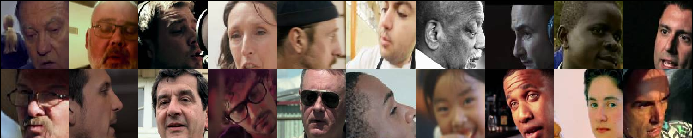
\includegraphics[width=0.98\linewidth]{img/random_selection_faces.pdf}
    \caption{A random selection of faces extracted from the dataset.}
    \label{fig:random_selection_faces}
\end{figure}

\section{Face similarity based on the deep features}

With respect to the results produces at \ref{}\todo{} we selected Dlib's model as model for computing the face features. The architecture of the network is based on the Resnet34 and trained on the mix of the available face datasets.

The network predicts into 128-dimensional space. We use the output of the network directly as our feature vectors. Note that, often face features refer to the specifics of the face landmarks, e.g., the color of the eyes, size of the lips and so on. To avoid confusion we use the term \emph{face encoding} for features obtained by pre-processing by neural network. Such face encoding is from space $\mathbb{R}^n$

After obtaining face encodings for our dataset of 2047 faces, we were interested, if this feature space created by the CNN is able to sort the faces based on the similarity in a similar way as people do. The library, from which we use the model, refers to a threshold 0.6 in euclidean distance for detecting, if two faces belong to the same person. The example of the closest faces based on this threshold is displayed in  figure \ref{fig:closest_faces}. In the provided example, we can see, that the face encodings close to our query face truly belong to the same person. Unfortunately, we can see, that with increasing distance other people appear even below the threshold 0.6.


\begin{figure}
    \centering
    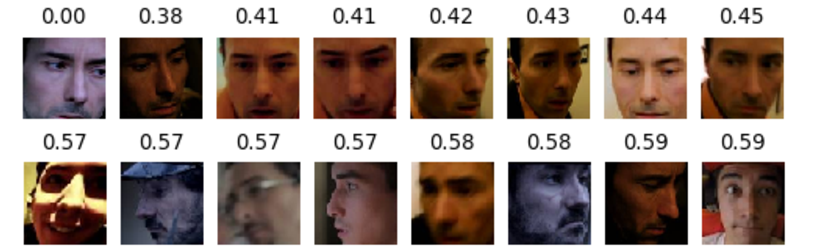
\includegraphics[width=\linewidth]{img/man_closest_faces.pdf}
    \caption{Examples of the retrieved closest faces to the query face (top left) based on euclidean distance. The number above each image represents the distance from the query.}
    \label{fig:closest_faces}
\end{figure}

\section{Case study}

The feature space with the distance we obtained from the model in the previous step was trained to perform well on the identification task. From the published results (\cite{}) we known that the model achieves state-of-art performance on the identification task. Therefore, we want to find out, if the space over the face features contains also information about the similarity between the faces. 

We conducted a study with 25 participants. We presented them a grid $10\times10$ of randomly selected faces from the dataset. 
Then we showed them 10 randomly selected target faces of different people. We asked the participant to select for each target face exactly three faces from the grid that looked the most similar. Out of 10 people in target images, one of them was a child and two others was presented in the grid.
%Then we asked them, to select exactly three faces, which are the most similar to the provided target face. Our test contained 10 randomly pre-selected faces of different people. Out of 10, one of them was a child, we estimate below 10 years old. Two of the other target faces were present in the grid.
One of them was extracted from the same image, i.e. the same angle of the face. The second of the target faces, which were shown in the grid, had two representants in the grid. One identical to the target face, the second one only with a minor change of the angle.

Twenty-four out of 25 respondents selected the face corresponding to the same target person in the first case. In the second case, two face views of the target person were available in the grid. 9 respondents selected both correctly and 11 respondents selected only one of them. We conclude, that only in 70.7\% of the cases users noticed the target person in the grid $10\times10$.

We further investigate the seven target faces, which were not present in the grid. For each of the faces from the grid we computed the Euclidean distance from the target face encoding to them. We then reordered the faces from the grid based on this distance. The closest faces received had the lowest index over the sorted distances. We refer to the index of the face in the sorted set of faces as $rank$.

We were interested in the distribution of ranks given the faces selected by the users. This would show us, if there is any correlation between similarity in the feature space and the similarity percieved by the human respondents. From the survey responses we create a heatmap for each task. The size of the heatmap corresponds to the size of the face grid, i.e., $10\times10$. The element on the position $task, i, j$ of the heatmap corresponds to the number of times, the face at $i$-th row and in $j$-th column was selected in the given $task$. We use the heatmap and the ranking based on the distances in the feature space, to compute, how many closest faces from feature space were actually selected. We do the same for each rank. The normalized results over all possible ranks (from 0 to 99) are plotted in the figure \ref{fig:survey_distribution}. If the users perception was fully coherent with the ordering based on the distances in the feature space, the  
probability on the first three ranks (0,1,2) would be equal to 1. Even though we do not see such full coherence in the results, we can see a trend of decreasing probability of choosing a face by user with the increasing distance from the target face.

We also show a comparison to the performing only six tasks, excluding the one, where the target person was child. The used network for feature extraction as many other are not performing well on the children from the dataset. This is caused by fact that most of the available face datasets contain only adults. This causes the networks to often put children closer together, even though, they may be a different person. Encodings of two different children tend to be closer to each other compared to the encoding of the two adults (source: \href{https://face-recognition.readthedocs.io/en/latest/readme.html#caveats}{Face Recognition Caveats}). Therefore we can see a significant improvement over the lowest ranks, since selecting a child from the map resulted in smaller distances, compared to the adults.

As the last investigation from the case study we provide a graph displaying the expected value of the number of faces selected up to a given rank (figure \ref{fig:random_selection_faces}). On average, one of the three selected by the user, has rank less than 12. Base on the user study we showed that this feature space over face encodings provides us with some information about face similarities.

\begin{figure}
    \centering
    \begin{subfigure}[b]{0.48\textwidth}
     \centering
     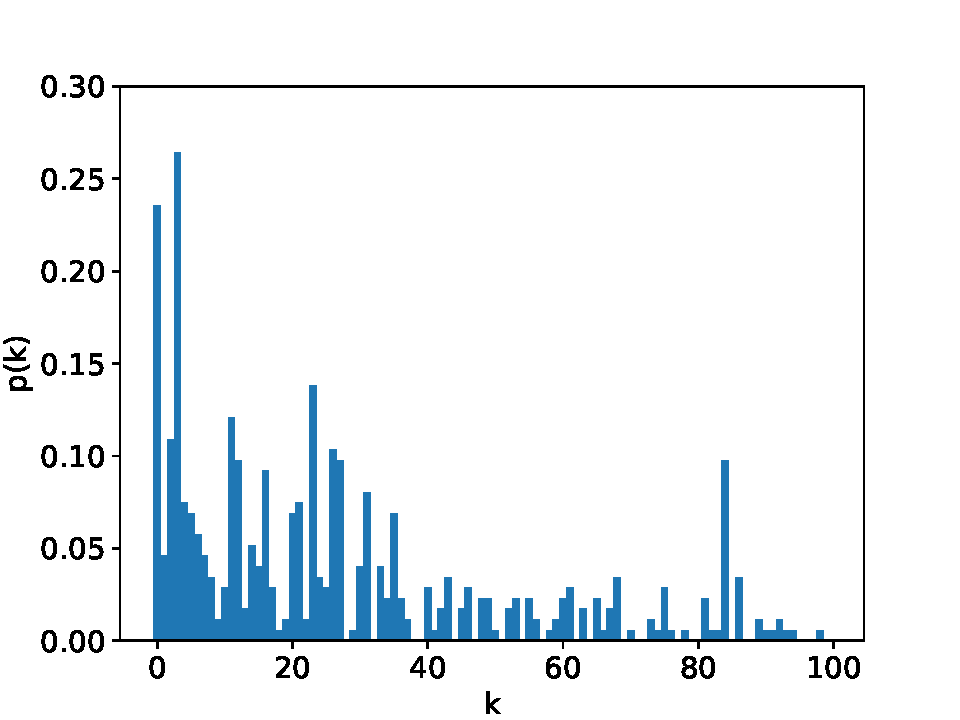
\includegraphics[width=\textwidth]{graphs/survey_distribution_without_the_easy.pdf}
     \caption{Performed on 7 task, which did not contain the target person in the grid}
     \label{fig:survey_all}
    \end{subfigure}
    \begin{subfigure}[b]{0.48\textwidth}
     \centering
     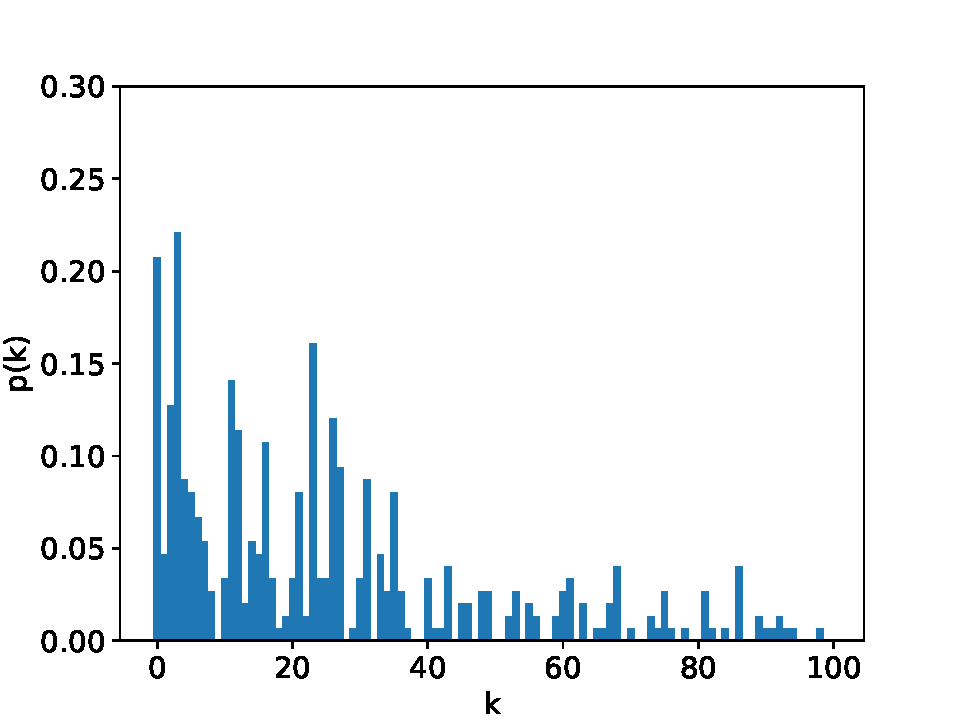
\includegraphics[width=\textwidth]{graphs/survey_distribution_childless.pdf}
     \caption{Performed on six tasks, extracting the task involving a child}
     \label{fig:suvery_childless}
    \end{subfigure}
    
    \caption{Collected statistic on how likely user selects $k$-th closest face to the target in the face grid. Ideally, if user was fully coherent with the distances in the features space, $p(k) = 1$ on [0, 2], since the user selected exactly 3 faces, and $p(k) = 0$ for all other $k$.}
    \label{fig:survey_distribution}
\end{figure}


\begin{figure}
    \centering
    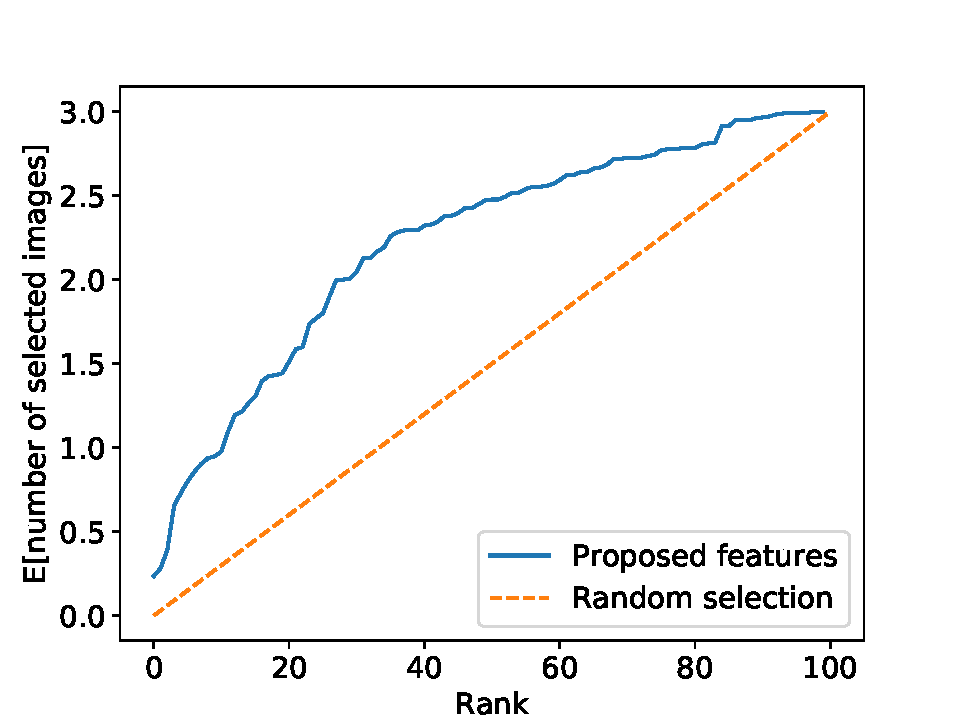
\includegraphics[width=0.8\linewidth]{graphs/survey_cumsum_without_the_easy.pdf}
    \caption{Expected value of the number of images selected up to a given rank. {\color{red} spis tested features ne?}}
    \label{fig:my_label}
\end{figure}

\section{Building a traversal scheme}

In the previous sections, we obtained and encoded faces. We investigated the feature space based on the correspondence to the manual annotations in the case study. Here we propose a solution of organizing faces into a multilevel view. 

As we discussed in Related Work, a common solution for traversal system is a 2D grid. This usually allows users navigation queries, as left, right, top, bottom. We call a set of images, which is visible at a prticular step a \emph{display}. Display may contain from tens to hundreds images at once depending on multiple factor, e.g. a user's screen size and a size of the displayed image.

Since most of the times, we want to display more data than low hundreds, it becomes inconvenient to preview dataset only in a one layer. Therefore, we build a simple multilevel structure to ease the navigation, when moving by a greater distance.

\subsection{Tree-based structure}

Our goal is to organise a dataset of images $D$. Let us assume, that the dataset can be organized into a grid of size $N\times M$. We leave the choice of the specific dimensions to the user. We prefer square setting, although, it is not required. In case, that the size of the dataset $|D|$ is almost a square of any number, we recommend adding a dummy images.

We organise (so far in non-specific way) the items from the dataset into a 2D grid. This is our base layer for the tree structure, we denote it as $L_0$. The overview of the structure is shown in the figure \ref{fig:tree_structure}. The layer has dimensions $L_{0, h}\times L_{0, w}$. Based on this layer, we create a next layer as only a subset of this layer. Firstly, we select a $k$, which represents the subset size factor. It means, that every $k^2$-th image is selected as a representant to the next layer

The layer $L_{i+1}$ has $1/k$ of the size in both axis of the $L_i$, more specifically, if the $L_i$ is of the dimensions $L_{i,h} \times L_{i,w}$, the layer $L_{i+1}$ has following dimensions:

$$
    L_{i+1, h} = \ceil*{L_{i, h} / k}
$$

$$
    L_{i+1, w} = \ceil*{L_{i, w} / k}
$$


The item on the position $m, n$ in the $L_{i+1}$ is replicated from the layer $L_i$ as follows:
$$
    L_{i+1, m, n} = L_{i, mk, nk} 
$$

We continue reducing the size of the layers, until the layer will fit to a display of user's screen.

In this structure we support six types of navigation: left, right, down, up, in, out. In and out represent operations between the layers and other directional commands navigate withing the layer. 


\begin{figure}
    \centering
    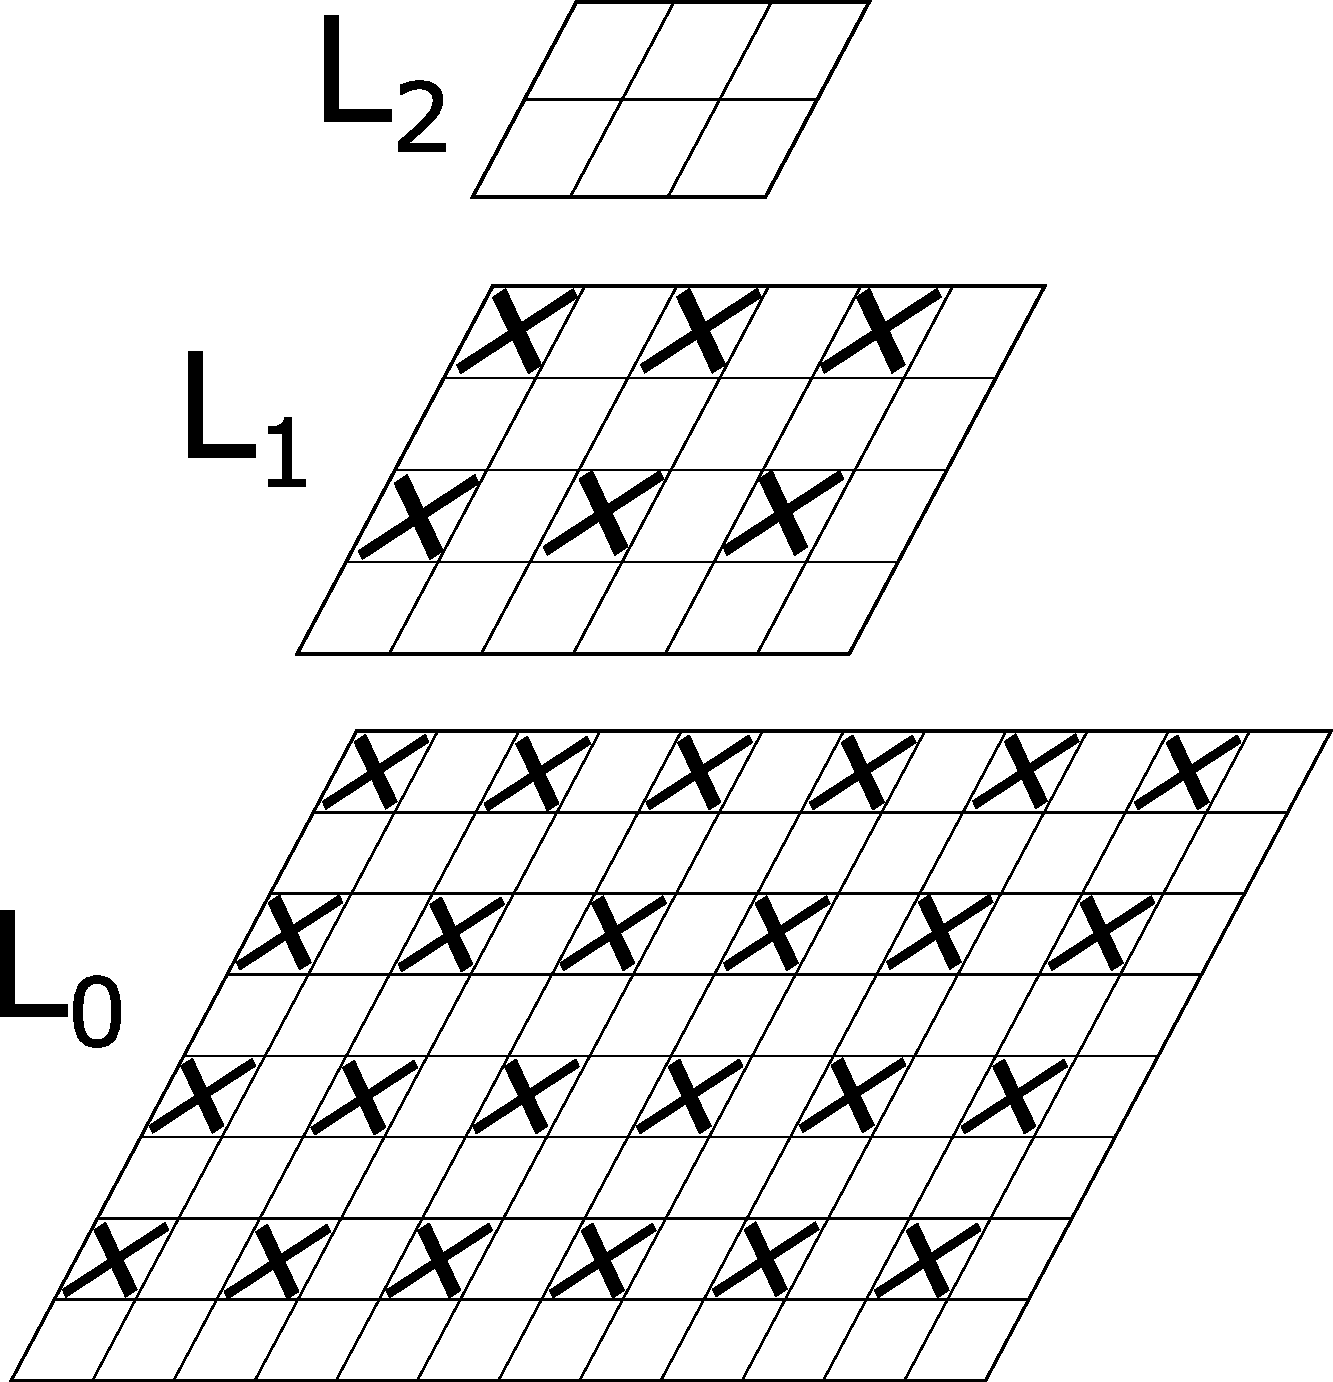
\includegraphics[width=0.3\linewidth]{img/tree-structure.pdf}
    \caption{A preview of the tree-based structure with $k = 2$ for previewing images. The marked items are selected for the layer above.}
    \label{fig:tree_structure}
\end{figure}

\subsection{Bottom Layer -- Self organizing map}

In the bottom layer, we would like to make use of the face encodings. As we reviewd in Related Work, Self-organizing maps have the power to project high-dimensional data into 2D space. We train a self-organizing map on our dataset of face encodings. For our particular dataset, we train a network of size $50\times 50$. This offers us 2500 slots at the lowest layer, having more slots than faces in the dataset.

We trained the SOM for \todo{}. After the training, we assign to the each node of the SOM closest face in the feature space. This way we assign each of SOM nodes one representant. We investigated the representans, now projected into a grid, and we can observe, that after the training, faces corresponding to the same person are clustered together. In some parts of the map, there are duplicites. It means, that the same face is used as representant in multiple nodes. We evaluated how many of the faces are represented in the displayed set. 1619 out of 2047 faces were matched to one of the SOM node. All the videos, that missing faces were extracted from, had in the layer at least one other presentant.

% jednak to neni som, ale vyber reprezentantov
% ze vidime pokope jednotlivych ludi


\subsection{Accessing the most similar faces}

We enhance the tree-structure to support displaying the most similar faces to a given face. In the bottom layer, this is partly covered by the representation based on the \acrshort{som}. Pictures of one person create small clusters, as well as pictures of people in glasses. Though, the neighbourhood of the face does not usually include all similar faces, and it can quickly transition to a new cluster.

In order to provide the user with ability to display the faces (with their original images), we support displaying the closest faces to any given face from the tree-based structure. The user can access it by clicking in the top right corner of any face. Based on this face, we provide all images, which contain a face, with encoding closer to the clicked face than a given threshold.



\section{Evaluation}

In this section we present evaluation of the proposed, navigational system. The goal of this chapter was to propose exploration method over the dataset of faces. Therefore, we evaluate it by conducting an experiment including a user.

The task for the user is to find a target face in the dataset. As our baseline, we construct the grid of the faces, in random order. For searching in this grid a user can only scroll up and down through the dataset. We then test our traversal structure. The hypothesis we aim to prove is, that our solution decreases the average time needed to find the target face compared to the search in random dataset.

For our experiment we use ten randomly selected faces. For each of them we let the user search for the face in the dataset. Respondent A firstly searches for the faces in the baseline approach, then using the traversal structure. Respondent B searches in the opposite order, firstly they work with the traversal structure, and then with the baseline.

We measured the time required to successfully find the target image. We obtained 20 measurements per approach. Respondent A was not able to retrieve a ``face 4'' in both any of the search engine. We set the limit for this task as 10 minutes.  Respondent B successfully retrieved target images for all provided faces.

Based on the experiment, we present results in the graph \ref{fig:search_time}. In case of both respondents, the median of the time required to solving the task was lower for the traversal search compared to the linear search. We also note that, the average on the other hand does not show any improvement, using the traversal search.

By the results, the traversal system did not performed strongly better, nor worse compared to the linear search. The traversial approach may still present a desired solution, when it comes to larger datasets. In such large datasets it may be impossible to go through all presented faces, one by one. The traversal search have an advantage of the interactive environment, where faces from several videos can be visually evaluated at once.



\begin{figure}
    \centering
    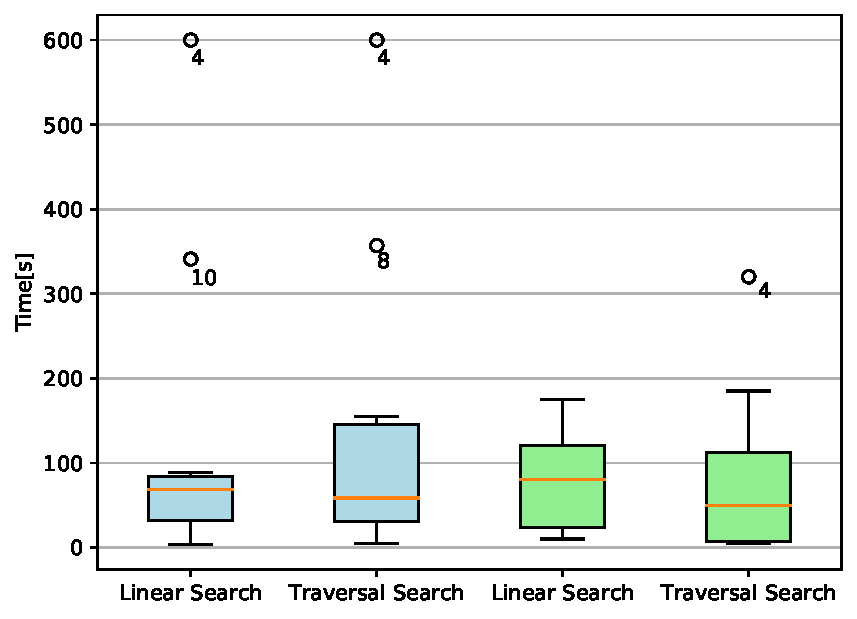
\includegraphics[width=0.7\linewidth]{graphs/face_search_time.pdf}
    \caption{Comparison of the time required to find a target image. Light blue belongs to the respondent A, light green to respondent B. The outliers are identified by the number of the query.}
    \label{fig:search_time}
\end{figure}